\newpage
\begin{flushright}
    \textbf{\Large{Ujian Tengah Semester}}
    \subsection*{Tahun 2023}
    \addcontentsline{toc}{subsection}{UTS - 2023}
\end{flushright}
\vspace{0.5cm}
\hrule height 2pt
\vspace{0.5cm}
\begin{center}
    \textbf{\large{MATERI}}
    \begin{enumerate}[leftmargin=*, label={\arabic*}.]
        \item Menyelesaikan pertidaksamaan yang melibatkan nilai mutlak.
        \item Mensketsa grafik fungsi.
        \item Menentukan range dan domain fungsi.
        \item Mencari nilai limit kiri dan nilai limit kanan fungsi.
        \item Menentukan kekontinuan fungsi pada suatu titik.
        \item Menyelesaikan masalah turunan implisit.
        \item Menyelesaikan permasalahan maksimum dan minimum.
        \item Menyelesaikan permasalahan laju yang berkaitan
    \end{enumerate}
\end{center}
\vspace{0.2cm}
\hrule height 1pt
\vspace{0.5cm}
\begin{center}
    \textbf{\large{SOAL}}
\end{center}
\begin{enumerate}[leftmargin=*, label={\arabic*}.]
\item Misalkan $\ds f(x) = \frac{\sqrt{5}\abs{x}}{x}$ dan $g(x) = -\sqrt{9-x^{2}}$.
\begin{enumerate}[label={\alph*}.]
    \item Tentukanlah domain dan range dari fungsi-fungsi tersebut!
    \item Tentukanlah himpunan penyelesaian dari: $f(x) \geq g(x)$.
\end{enumerate}
\item Diberikan fungsi $f$ dengan $f(x) = \floor{x}^2$.
\begin{enumerate}[label={\alph*}.]
    \item Sketsalah grafik fungsi $f$ tersebut!
    \item Tentukanlah
    \begin{enumerate}[label={\roman*}.]
        \item $f(-1)$
        \item $\ds\lim_{x\to -1^{+}} f(x)$
        \item $\ds\lim_{x\to -1^{-}} f(x)$
        \item $\ds\lim_{x\to -1} f(x)$
    \end{enumerate}
    \item Apakah fungsi $f$ kontinu di $x=-1$? Jelaskanlah!
    \item Jika $f$ tidak kontinu di $x=-1$, apakah ketidakkontinuan tersebut bisa 
    diperbaiki? Jelaskanlah!
\end{enumerate}
\item Carilah persamaan garis singgung dari kurva $(x^2+y^2)^2=(x-y)^2$ di titik $(1,-1)$.
\item Diketahui sebuah fungsi $f$ memenuhi \textbf{semua} kondisi berikut:
\begin{itemize}
    \item $f$ kontinu dimana-mana,
    \item $f(1)=2,f(2)=1,f(4)=4,f(6)=7,f(8)=3$,
    \item $f'(2)=0,f'(4)=1,f'(6)$ dan $f'(8)$ tidak ada,
    
    $f'(x)<0$ untuk $x < 2$ atau $x>6$, $f'(x)>0$ untuk $2<x<6$,
    \item $f''(4) = 0$, $f''(x)<0$ untuk $4<x<6$ atau $x > 8$,
    
    $f''(x)>0$ untuk $x<4$ atau $6 < x < 8$.
\end{itemize}
\begin{enumerate}[label={\alph*}.]
    \item Di interval manakah fungsi tersebut naik atau turun, cekung ke atas atau 
    ke bawah? Apakah grafik fungsi tersebut mempunyai titik belok 
    (\textit{inflextion point})? Jelaskanlah!
    \item Tentukanlah titik-titik kritis dari fungsi $f$ pada interval 
    $\cio*{1,\infty}$. Kemudian tentukanlah nilai maksimum dan minimum dari fungsi $f$ 
    pada interval tersebut (jika ada)!
    \item Buatlah sketsa grafik fungsi tersebut!
    \item Apakah terdapat bilangan $c$ dalam interval $\cic*{1,6}$ yang memenuhi 
    Teorema Nilai Rata-rata untuk Turunan? Jelaskanlah! Jika ada, tentukanlah \textbf{semua} 
    bilangan $c$ tersebut.
\end{enumerate}
\item Seseorang $(A)$ berdiri di tepi sungai mengamati perahu yang melintas (seperti pada 
gambar di bawah). Asumsikan posisi perahu saat melaju selalu tepat di tengah sungai. Diketahui 
lebar sungai adalah $12$ meter. Jika sudut pengamatan antar $A$ dengan perahu adalah 
$\theta =\frac{\pi}{3}$rad dan kecepatan perubahan sudut $\theta$ adalah $3$rad/detik, berapa 
kecepatan perahu pada saat itu?
\vspace{0.2cm}
\begin{center}
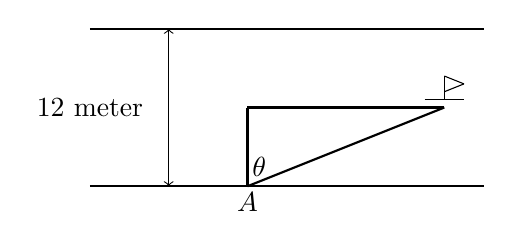
\begin{tikzpicture}
    \draw[thick] (-2,1)--(3,1);
    \draw[thick] (-2,-1)--(3,-1);
    \draw[thin, <->] (-1,-1)--(-1,1);
    \draw[thick] (0,-1)--(0,0);
    \draw[thick] (0,0)--(2.5,0);
    \draw[thick] (0,-1)--(2.5,0);
    \draw[thin] (2.25,0.1)--(2.75,0.1);
    \draw[thin] (2.5,0.1)--(2.5,0.4);
    \draw[thin] (2.75,0.3)--(2.5,0.4);
    \draw[thin] (2.75,0.3)--(2.5,0.2);
    
    \node at (-2,0) {$12$ meter};
    \node at (0.15,-0.75) {$\theta$};
    \node at (0,-1.2) {$A$};
    \end{tikzpicture}
\end{center}
\end{enumerate}
\vspace{0.2cm}
\hrule height 1pt
\vspace{0.5cm}
\begin{center}
    \textbf{\large{PEMBAHASAN}}
\end{center}
\begin{enumerate}[leftmargin=*, label={\arabic*}.]
\item Diberikan fungsi $\ds f(x) = \frac{\sqrt{5}\abs{x}}{x}$ dan $g(x) = -\sqrt{9-x^{2}}$.
\begin{enumerate}[label={\alph*}.]
    \item Pertama akan dicari domain dan range dari $f$.
    
    Untuk domainnya, karena $f$ memiliki bentuk rasional, maka penyebut tidak boleh nol. 
    Sehingga domain natural $f$ adalah bilangan real selain nol.\\
    Untuk rangenya, karena melibatkan bilangan mutlak $|x|$ dapat dilakukan pembagian 
    kasus untuk menghilangkan bentuk mutlaknya.\\
    Untuk $x>0$ maka
    \[
        \frac{\sqrt{5}\abs{x}}{x} = \frac{\sqrt{5}x}{x} = \sqrt{5}
    \]
    dan untuk $x < 0$ maka
    \[
        \frac{\sqrt{5}\abs{x}}{x} = \frac{\sqrt{5}(-x)}{x} = -\sqrt{5}
    \]
    sehingga range dari $f$ adalah $\sqrt{5}$ dan $-\sqrt{5}$.

    Diperoleh domain dari $f$ adalah $D_f=\set*{x\in \mathbb{R} \mid x\neq 0}$ dan 
    range $R_f=\set*{\sqrt{5},-\sqrt{5}}$

    Kedua akan dicari domain dan range dari $g$.

    Untuk domainnya, karena $g$ memiliki bentuk akar kuadrat, maka $9-x^{2}$ harus nonnegatif.\\
    Selesaikan pertidaksamaan berikut
    \[
        9-x^{2} \geq 0 \iff x^{2}-9 \leq 0 \iff (x+3)(x-3) \leq 0
    \]
    Maka titik stasionernya adalah $x=3$ dan $x=-3$.
    \begin{center}
    \begin{tikzpicture}
        \draw[stealth-stealth] (-5,0) node[below]{$-\infty$}--(5,0) node[below]{$\infty$};
        \draw (2,1) --(-2,1);
        \draw (-2,1)--(-2,-.1) node[below=0.2em]{$-3$};
        \draw (2,1)--(2,-.1) node[below=0.2em]{$3$};
                
        \node at (-3.5,.5) {$+$};
        \node at (0,.5) {$-$};
        \node at (3.5,.5) {$+$};
        \node [draw, shape = circle, fill = black, minimum size = 0.1cm, inner sep=0pt] at (2,0){};
        \node [draw, shape = circle, fill = black, minimum size = 0.1cm, inner sep=0pt] at (-2,0){};
        \end{tikzpicture}
    \end{center}
    Diperoleh domain dari $g$ adalah bilangan real $x$ dengan $-3 \leq x \leq 3$.

    Untuk range dari $g$, karena akar kuadrat selalu bernilai nonnegatif, maka kebalikannya selalu 
    nonpositif. Batas atas range fungsi $g$ adalah $0$. Untuk batas bawahnya akan dicari nilai minimum 
    dari $g$. Carilah titik stasioner $g$ pada domainnya.
    \begin{align*}
        g'(x) = 0 \iff &\drv{x}{-\sqrt{9-x^{2}}} = 0\\
        \iff &-\frac{1}{2}\frac{1}{\sqrt{9-x^{2}}}\drv{x}{9-x^{2}}=0\\
        \iff &\frac{x}{\sqrt{9-x^{2}}} = 0\\
        \iff & x=0
    \end{align*}
    Subtitusi $x=0$ ke $g$ diperoleh $g(0) = -\sqrt{9-0^{2}} = -\sqrt{9}=-3$. Ini adalah batas 
    bawah range $g$. Sehingga diperoleh range dari $g$ adalah $-3 \leq y \leq 0$.

    $\therefore$ Domain dan range dari $f$ adalah $D_f=\set*{x\in \mathbb{R} \mid x\neq 0}$ dan 
    $R_f=\set*{\sqrt{5},-\sqrt{5}}$ juga domain dan range dari $g$ adalah 
    $D_g=\set*{x\in \mathbb{R} \mid -3 \leq x \leq 3}$ dan 
    $R_g=\set*{y\in \mathbb{R} \mid -3 \leq x \leq 0}$.

\begin{center}
    \line(1,0){150}
\end{center}

    \item Akan dicari himpunan penyelesaian dari $\ds f(x) \geq g(x) 
    \iff \frac{\sqrt{5}\abs{x}}{x} \geq -\sqrt{9-x^{2}}$.

    Syarat dari kedua ruas mengharuskan nilai $x$ memenuhi kedua domain $f$ dan $g$. 
    Sehingga himpunannya penyelesaiannya hanya diantara $\cic{-3,3} \cap x \neq 0$.
    Bagi kasus untuk menghilangkan bentuk nilai mutlak.

    \textbf{Kasus 1: $0 < x \leq 3$}\\
    Maka
    \begin{align*}
        \frac{\sqrt{5}\abs{x}}{x} \geq -\sqrt{9-x^{2}}
        \iff &\frac{\sqrt{5}x}{x} \geq -\sqrt{9-x^{2}} 
        &\text{definisi nilai mutlak} \\
        \iff &\sqrt{5} \geq -\sqrt{9-x^{2}}
        &\text{penyederhanaan}
    \end{align*}
    $\sqrt{5}>0$ dan $-\sqrt{9-x^{2}} \leq 0$, sehingga pertidaksamaan diatas selalu 
    bernilai benar. Sehingga pada kasus ini himpunan penyelesaiannya adalah $0 < x \leq 3$.

    \textbf{Kasus 2: $-3 \leq x < 0$}\\
    Maka
    \begin{align*}
        \frac{\sqrt{5}\abs{x}}{x} \geq -\sqrt{9-x^{2}}
        \iff &\frac{\sqrt{5}(-x)}{x} \geq -\sqrt{9-x^{2}} 
        &\text{definisi nilai mutlak} \\
        \iff &-\sqrt{5} \geq -\sqrt{9-x^{2}}
        &\text{penyederhanaan}\\
        \iff &\sqrt{5} \leq \sqrt{9-x^{2}}
        &\text{kedua ruas kalikan $-1$}\\
        \iff & 5 \leq 9-x^{2}
        &\text{kuadratkan kedua ruas}\\
        \iff &x^{2}-4 \leq 0
        &\text{kedua ruas jumlahkan $x^{2}-9$}\\
        \iff &(x+2)(x-2) \leq 0
    \end{align*}
    Maka titik stasionernya adalah $x=-2$ dan $x=2$.
    \begin{center}
        \begin{tikzpicture}
            \draw[stealth-stealth] (-5,0) node[below]{$-\infty$}--(5,0) node[below]{$\infty$};
            \draw (2,1) --(-2,1);
            \draw (-2,1)--(-2,-.1) node[below=0.2em]{$-2$};
            \draw (2,1)--(2,-.1) node[below=0.2em]{$2$};
                    
            \node at (-3.5,.5) {$+$};
            \node at (0,.5) {$-$};
            \node at (3.5,.5) {$+$};
            \node [draw, shape = circle, fill = black, minimum size = 0.1cm, inner sep=0pt] at (2,0){};
            \node [draw, shape = circle, fill = black, minimum size = 0.1cm, inner sep=0pt] at (-2,0){};
            \end{tikzpicture}
        \end{center}
    Pada kasus ini nilai $x$ yang memenuhi adalah $-2 \leq x \leq 2$. Iriskan dengan syarat 
    pada kasus ini diperoleh himpunan penyelesaiannya adalah $-2 \leq x < 0$.

    Gabungkan kedua kasus tersebut untuk memperoleh himpunannya penyelesaiannya \\
    $\set*{x \in \mathbb{R} \mid -2 \leq x < 0 \cup 0 < x \leq 3}$.

    $\therefore$ Diperoleh himpunan penyelesaian dari $\ds f(x) \geq g(x)$ adalah 
    $\set*{x \in \mathbb{R} \mid -2 \leq x < 0 \cup 0 < x \leq 3}$.
\begin{center}
    \line(1,0){300}
\end{center}
\end{enumerate}
\item Diberikan fungsi $f(x) = \floor{x}^2$.
\begin{enumerate}[label={\alph*}.]
    \item Sketsa fungsi tangga $\floor{x}$ lalu kuadratkan masing-masing \textit{step} 
    untuk memperoleh $\floor{x}^{2}$.
\begin{center}
\begin{tikzpicture}[>=stealth]
\begin{axis}[
    xmin=-5.5,xmax=5.5,
    ymin=-5.5,ymax=5.5,
    axis x line=middle,
    axis y line=middle,
    axis line style=<->,
    xlabel={$x$},
    ylabel={$y$},
    ]
    \foreach \n in {-5,...,4} {
        \addplot[no marks,blue, -] expression[domain={\n}:{\n+1},samples=10]{floor(\n)}
            node[draw, shape = circle, fill = white, minimum size = 0.1cm, inner sep=0pt]{}
            node[pos=0, draw, shape = circle, fill = blue, minimum size = 0.1cm, inner sep=0pt]{};
    }
    \node[blue] at (2,4){$y=\floor{x}$};
\end{axis}
\end{tikzpicture}\\
\begin{tikzpicture}[>=stealth]
    \begin{axis}[
        xmin=-5.5,xmax=5.5,
        ymin=-0.5,ymax=20,
        axis x line=middle,
        axis y line=middle,
        axis line style=<->,
        xlabel={$x$},
        ylabel={$y$},
        ]
        \foreach \n in {-5,...,4} {
            \addplot[no marks,red, -] expression[domain={\n}:{\n+1},samples=10]{floor(\n)^2}
                node[draw, shape = circle, fill = white, minimum size = 0.1cm, inner sep=0pt]{}
                node[pos=0, draw, shape = circle, fill = red, minimum size = 0.1cm, inner sep=0pt]{};
        }
        \node[red] at (2,15){$y=\floor{x}^2$};
    \end{axis}
    \end{tikzpicture}
\end{center}

    $\therefore$ Telah disketsa grafik $f$.
\begin{center}
    \line(1,0){150}
\end{center}
    \item Pada $x=-1$ 
    \begin{enumerate}[label={\roman*}.]
        \item Akan dicari $f(-1)$.
        \[
        f(-1) = \floor{-1}^{2} = (-1)^{2} = 1
        \]
        $\therefore$ Diperoleh $f(-1)=1$.
\begin{center}
    \line(1,0){150}
\end{center}
        \item Akan dicari $\ds\lim_{x\to -1^{+}} f(x)$
        
        Perhatikan grafik pada jawaban sebelumnya. Saat fungsi menuju $x=-1$ dari kanan, nilai 
        limitnya akan menuju $1$.

        $\therefore$ Diperoleh $\ds\lim_{x\to -1^{+}} f(x) = 1$.
\begin{center}
    \line(1,0){150}
\end{center}
        \item Akan dicari $\ds\lim_{x\to -1^{-}} f(x)$
        
        Perhatikan grafik pada jawaban sebelumnya. Saat fungsi menuju $x=-1$ dari kiri, nilai 
        limitnya akan menuju $4$.

        $\therefore$ Diperoleh $\ds\lim_{x\to -1^{-}} f(x) = 4$.
\begin{center}
    \line(1,0){150}
\end{center}
        \item Akan dicari $\ds\lim_{x\to -1} f(x)$
        
        Dari kedua hasil sebelumnya, diperoleh nilai limit kanan dan limit kiri yang berbeda saat 
        $x$ menuju $-1$. Dengan demikian nilai limitnya tidak ada.

        $\therefore$ Diperoleh $\ds\lim_{x\to -1} f(x)$ tidak ada.
\begin{center}
    \line(1,0){150}
\end{center}
    \end{enumerate}
    \item Tiga syarat untuk membuktikan $f$ kontinu di $x=-1$ adalah
    \begin{enumerate}[label={\arabic*}.]
        \item $\lim_{x\to -1} f(x)$ ada.
        \item $f(-1)$ ada.
        \item $\lim_{x\to -1} f(x) = f(-1)$
    \end{enumerate}

    Jawaban sebelumnya telah menunjukkan bahwa $\lim_{x\to -1} f(x)$ tidak ada. Dengan 
    demikian $f$ tidak kontinu di $x=-1$.

    $\therefore$ $f$ tidak kontinu di $x=-1$ karena $\lim_{x\to -1} f(x)$ tidak ada.
\begin{center}
    \line(1,0){150}
\end{center}
    \item Ketidakkontinuan dapat diperbaiki dengan mendefinisikan ulang nilai $f$ di $x=-1$ dengan 
    nilai limitnya. Karena $\lim_{x\to -1} f(x)$ tidak ada maka ketidakkontinuannya tidak dapat 
    diperbaiki.

    $\therefore$ Ketidakkontinuan $f$ di $x=-1$ tidak dapat diperbaiki.
\end{enumerate}
\begin{center}
    \line(1,0){300}
\end{center}
\item Akan dicari persamaan garis singgung dari kurva $(x^2+y^2)^2=(x-y)^2$ di titik $(1,-1)$.

Untuk memperoleh persamaan garis singgung, maka diperlukan titik singgung dan kemiringannya.
Akan dicari kemiringan garis singgung dari kurva $(x^2+y^2)^2=(x-y)^2$ di titik $(1,-1)$ dengan 
menggunakan turunan pertama.

Turunkan secara implisit persamaan kurva lalu subtitusikan $x=1$ dan $y=-1$.
\begin{align*}
    &\drv{x}{\brk*{x^{2}+y^{2}}^{2}} = \drv{x}{(x-y)^{2}}\\
    \iff &2\brk*{x^{2}+y^{2}}\drv{x}{x^{2}+y^{2}} = 2(x-y)\drv{x}{x-y}
    &\text{aturan rantai}\\
    \iff &2\brk*{x^{2}+y^{2}}(2x+2yy') = 2(x-y)(1-y')\\
    &2((1)^{2}+(-1)^{2})(2(1)+2(-1)y') = 2(1-(-1))(1-y')
    &\text{subtitusi $x=1$ dan $y=-1$}\\
    \iff &2(2)(2-2y')=2(2)(1-y')\\
    \iff & 2-2y'=1-y'\\
    \iff & y'=1
\end{align*}
Diperoleh kemiringan $m=y'=1$ pada titik $(1,-1)$.
Masukan kedalam persamaan garis singgung diperoleh
\begin{align*}
    y-y_{1} = m(x-x_{1}) &\iff y-(-1)=1(x-1)\\
    &\iff y+1 = x-1\\
    &\iff x-y-2=0 
\end{align*}

$\therefore$ Persamaan garis singgung dari kurva $(x^2+y^2)^2=(x-y)^2$ di titik $(1,-1)$ adalah 
$x-y-2=0$
\begin{center}
    \line(1,0){300}
\end{center}
\item Diberikan sebuah fungsi $f$ memenuhi \textbf{semua} kondisi berikut:
\begin{itemize}
    \item $f$ kontinu dimana-mana,
    \item $f(1)=2,f(2)=1,f(4)=4,f(6)=7,f(8)=3$,
    \item $f'(2)=0,f'(4)=1,f'(6)$ dan $f'(8)$ tidak ada,
    
    $f'(x)<0$ untuk $x < 2$ atau $x>6$, $f'(x)>0$ untuk $2<x<6$,
    \item $f''(4) = 0$, $f''(x)<0$ untuk $4<x<6$ atau $x > 8$,
    
    $f''(x)>0$ untuk $x<4$ atau $6 < x < 8$.
\end{itemize}
\begin{enumerate}[label={\alph*}.]
    \item Pertama akan ditentukan interval dimana fungsi tersebut naik dan turun.
    
    Interval dimana fungsi naik adalah untuk nilai $x$ dimana $f'(x) > 0$ dan turun 
    untuk nilai $x$ dimana $f'(x) < 0$. Dari poin ketiga, terlihat bahwa fungsi $f$ 
    naik pada interval $\oio{2,6}$ dan turun pada interval 
    $\oio{-\infty,2} \cup \oio{6,\infty}$.
    
    Kedua akan ditentukan interval dimana fungsi tersebut cekung ke atas dan ke bawah.

    Interval dimana fungsi cekung ke atas adalah untuk nilai $x$ dimana $f''(x) > 0$ 
    dan cekung ke bawah untuk nilai $x$ dimana $f''(x) < 0$. Dari poin keempat, terlihat 
    bahwa fungsi $f$ cekung ke atas pada interval 
    $\oio{-\infty,4} \cup \oio{6,8}$ dan cekung ke bawah pada interval 
    $\oio{4,6} \cup \oio{8,\infty}$.

    Ketiga akan dicari titik belok fungsi tersebut (jika ada).

    Titik belok adalah titik dimana di satu sisi fungsi tersebut cekung ke atas dan 
    di sisi lainnya fungsi tersebut cekung ke bawah. Dari poin keempat, terlihat bahwa 
    ada tiga titik belok yaitu $x=4$ (dari atas ke bawah), $x=6$ (dari bawah ke atas) 
    dan $x=8$ (dari atas ke bawah).

    $\therefore$ $\oio{2,6}$ adalah interval dimana $f$ naik, 
    $\oio{-\infty,2} \cup \oio{6,\infty}$ adalah interval dimana $f$ 
    turun, $\oio{-\infty,4} \cup \oio{6,8}$ adalah interval dimana $f$ 
    cekung ke atas, $\oio{4,6} \cup \oio{8,\infty}$ adalah interval 
    dimana $f$ cekung ke bawah dan $x=4,6,8$ adalah titik belok fungsi $f$.
\begin{center}
    \line(1,0){150}
\end{center}
    \item Akan dicari titik-titik kritis dari fungsi $f$ di interval $\cio{1,\infty}$.\\
    Titik kritis terjadi pada
    \begin{enumerate}[label={\arabic*})]
        \item Ujung interval
        \item Titik stasioner (saat $f'(c)=0$)
        \item Titik singular (saat $f'(c)$ tidak ada)
    \end{enumerate}
    Dengan demikian $x=1$ sebagai ujung interval adalah titik kritis. Dari poin ketiga $x=2$ 
    adalah titik stasioner (karena $f'(2)=0$), lalu $x=6$ dan $x=8$ adalah titik singular 
    (karena $f'(6)$ dan $f'(8)$ tidak ada). Sehingga diperoleh titik-titik kritis $x=1$, $x=2$, 
    $x=6$ dan $x=8$.

    Nilai maksimum dan minimum hanya terjadi di titik kritis. Disini dapat diuji masing-masing 
    titik kritis
    \[
        f(1) = 2, \quad f(2)=1, \quad f(6) =7, \quad f(8) = 3
    \]
    Dari keempat nilai ini maka $f(2)=1$ dan $f(6)=7$ adalah nilai ekstrim, hal ini karena fungsi $f$ 
    turun sebelum $x=2$ dan naik setelah $x=2$ dan fungsi $f$ naik sebelum $x=6$ dan turun setelah 
    $x=6$. Karena fungsi $f$ kontinu di $\cio{1,\infty}$ dan $f$ turun untuk $x>8$ maka 
    $f$ tidak memiliki nilai minimum sedangkan titik $x=6$ akan menjadi titik maksimum $f$ di 
    $\cio{1,\infty}$. \\
    (Untuk lebih jelas dapat dilihat visualisasi sketsa $f$ di soal 
    berikutnya).

    $\therefore$ Titik-titik kritis dari fungsi $f$ di interval $\cio{1,\infty}$ adalah 
    $x=1$, $x=2$, $x=6$ dan $x=8$. Pada interval tersebut, $f$ memiliki nilai maksimum $f(6)=7$ 
    dan tidak memiliki nilai minimum.

    \item Gunakan informasi hasil dari soal sebelumnya untuk membantu sketsa grafik $f$.\\
    Berikut sketsa ilustrasi fungsi $f$ dengan kondisi yang diberikan.
    \begin{center}
    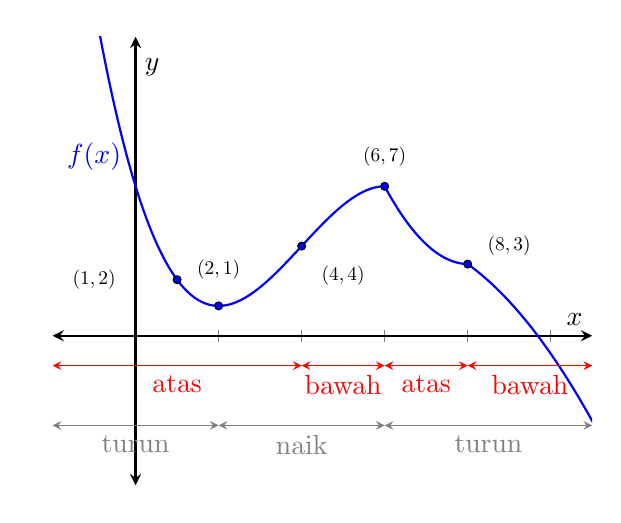
\begin{tikzpicture}[>=stealth]
    \begin{axis}[
        xmin=0,xmax=6.5,
        ymin=-5,ymax=10,
        axis x line=middle,
        axis y line=middle,
        y axis line style={draw=none},
        x axis line style={thick},
        y tick style={draw=none},
        axis line style=<->,
        yticklabel=\empty,
        xticklabel=\empty,
        xlabel={$x$},
        ]
        \draw[thick, <->] (1,10) -- (1,-5);
        \addplot[no marks,blue, thick, -] expression[domain=0:4,samples=200]{-(x-2)^3+3*(x-2)^2+1};
        \addplot[no marks,blue, thick, -] expression[domain=4:5,samples=200]{(1.5969*x-8)^2+2.4};
        \addplot[no marks,blue, thick, -] expression[domain=5:8,samples=200]{-(x-4)^2+3.4};
        \node [draw, shape = circle, fill = blue, minimum size = 0.1cm, inner sep=0pt] at (2,1){};
        \node at (2,2.2){\scalebox{0.7}{$(2,1)$}};
        \node [draw, shape = circle, fill = blue, minimum size = 0.1cm, inner sep=0pt] at (1.5,1.875){};
        \node at (0.5,1.875){\scalebox{0.7}{$(1,2)$}};
        \node [draw, shape = circle, fill = blue, minimum size = 0.1cm, inner sep=0pt] at (3,3){};
        \node at (3.5,2){\scalebox{0.7}{$(4,4)$}};
        \node [draw, shape = circle, fill = blue, minimum size = 0.1cm, inner sep=0pt] at (4,5){};
        \node at (4,6){\scalebox{0.7}{$(6,7)$}};
        \node [draw, shape = circle, fill = blue, minimum size = 0.1cm, inner sep=0pt] at (5,2.4){};
        \node at (5.5,3){\scalebox{0.7}{$(8,3)$}};
        \node at (1.2,9){{$y$}};
        \node[blue] at (0.5,6){{$f(x)$}};
        \draw[red, <->] (0,-1) -- node[below](){atas} (3,-1);
        \draw[red, <->] (3,-1) -- node[below](){bawah} (4,-1);
        \draw[red, <->] (4,-1) -- node[below](){atas} (5,-1);
        \draw[red, <->] (5,-1) -- node[below](){bawah} (6.5,-1);
        \draw[gray, <->] (0,-3) -- node[below](){turun} (2,-3);
        \draw[gray, <->] (4,-3) -- node[below](){turun} (6.5,-3);
        \draw[gray, <->] (2,-3) -- node[below](){naik} (4,-3);
    \end{axis}
    \end{tikzpicture}
    \end{center}

    $\therefore$ Telah disketsa grafik $f$.
\begin{center}
    \line(1,0){150}
\end{center}
    \item Akan dibuktikan teorema Nilai Rata-rata untuk Turunan berlaku dengan interval $\cic*{1,6}$.\\
    Syarat teorema ini adalah fungsi $f$ kontinu di $\cic*{1,6}$ dan terturunkan di $\oio*{1,6}$. 
    Poin pertama soal mengatakan $f$ kontinu dimana-mana sehingga $f$ juga kontinu di $\cic*{1,6}$. 
    Selanjutnya dari poin ketiga $f$ terturunkan dimana-mana kecuali di $x=6$ dan $x=8$, sehingga 
    jelas $f$ terturunkan di interval $\oio*{1,6}$. Karena telah memenuhi dua syarat teorema 
    maka dapat dipastikan terdapat nilai $c$ yang dimana (sesuai teorema):
    \[
    \frac{f(6)-f(1)}{6-1} = f'(c) \iff \frac{7-2}{5} = f'(c) \iff f'(c) = 1
    \]
    Akan dicari \textbf{semua} bilangan $c$ di $\oio*{1,6}$ sehingga $f'(c)=1$. \\Dari poin ketiga 
    soal didapat $f'(4)=1$.\\
    Akan ditunjukan hanya $c=4$ yang memenuhi:
    \begin{itemize}
        \item Karena $x=2$ adalah minimum lokal dan $f$ cekung atas di $\oio*{1,2}$ 
        maka $f'(x) < 0$ untuk semua $x$ di $\oio*{1,2}$
        \item $f'(2)=0 \neq 1$.
        \item Karena $x=4$ titik belok dengan $f'(4)=1$, lalu $f$ cekung atas di $\oio*{2,4}$ dan cekung bawah 
        di $\oio*{4,6}$ maka $f'(x) < 1$ untuk semua $x$ di $\oio*{2,6}, x\neq 4$.
    \end{itemize}
    Sehingga hanya $c=4$ yang memenuhi $f'(c)=1$.
    
    $\therefore$ Terdapat nilai $c$ yang memenuhi teorema Nilai Rata-rata untuk Turunan di interval $\cic*{1,6}$ 
    dan nilai tersebut hanya $c=4$.
\end{enumerate}

\vspace{0.1cm}
\textbf{Catatan:}\\
Apabila sudah mempelajari \textit{Analisis Real}, dapat dibuktikan fungsi diatas seharusnya tidak 
ada (kondisi yang diberikan berkontradiksi). Sketsa pada soal 4c hanyalah ilustrasi 
($f'(4)\neq 1$ pada sketsa tersebut).
\begin{center}
    \line(1,0){300}
\end{center}

\item Misalkan $x$ adalah perpindahan. 

Diberikan kecepatan gerak perahu dalam perubahan sudut 
sebagai $\ds\frac{d\theta}{dt} = 3$ rad/detik. 

Akan dicari $\ds\frac{dx}{dt}$ saat 
$\ds\theta = \frac{\pi}{3}$ rad.

Carilah hubungan antara $x$ dengan $\theta$.
\vspace{0.2cm}
\begin{center}
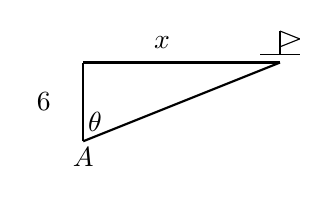
\begin{tikzpicture}
    \draw[thick] (0,-1)--(0,0);
    \draw[thick] (0,0)--(2.5,0);
    \draw[thick] (0,-1)--(2.5,0);
    \draw[thin] (2.25,0.1)--(2.75,0.1);
    \draw[thin] (2.5,0.1)--(2.5,0.4);
    \draw[thin] (2.75,0.3)--(2.5,0.4);
    \draw[thin] (2.75,0.3)--(2.5,0.2);
    
    \node at (-0.5,-0.5) {$6$};
    \node at (1,0.25) {$x$};
    \node at (0.15,-0.75) {$\theta$};
    \node at (0,-1.2) {$A$};
    \end{tikzpicture}
\end{center}
Terlihat bahwa saat $\theta = \pi/3$ diperoleh
\[
\tan \theta = \frac{x}{6} \iff x = 6\tan\theta
\]
Turunkan keduanya terhadap waktu
\[
\drv{t}{x} = \drv{t}{6\tan\theta} \iff \frac{dx}{dt} = 6\sec^{2}\theta\frac{d\theta}{dt}
\]
Subtitusi nilai $\theta = \pi/3$ dan $\frac{d\theta}{dt}=3$ sehingga
\[
\frac{dx}{dt} = 6\sec^{2}\brk*{\frac{\pi}{3}}(3) = 6(2)^{2}3 = 72
\]
Sehingga kecepatan perahu saat itu adalah $72$ meter/detik.

$\therefore$ Diperoleh kecepataan perahu saat itu adalah $72$ meter/detik.

\end{enumerate}

\begin{center}
    \line(1,0){300}
\end{center}